\usetikzlibrary{plotmarks}

\begin{figure}
\centering
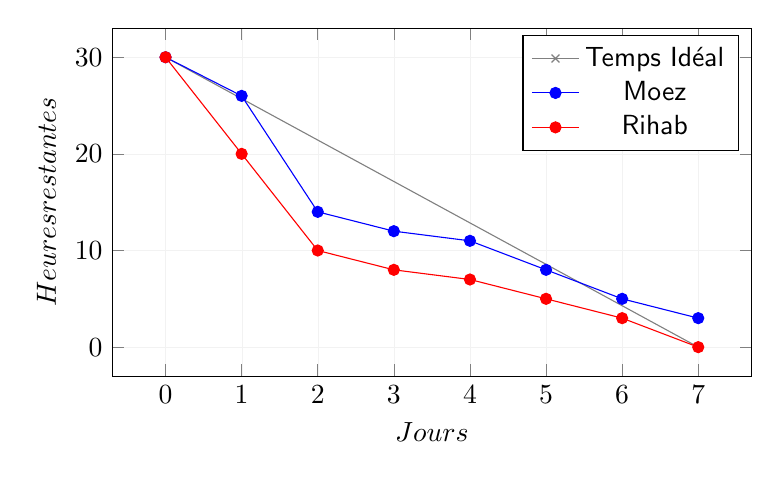
\begin{tikzpicture}[y=.2cm, x=.7cm,font=\sffamily]
\begin{axis}[
xlabel=$Jours$,
ylabel=$Heures restantes$,
grid=both,
grid style={line width=.1pt, draw=gray!10},
width=0.8\textwidth,
height=6cm,
%major grid style={line width=.2pt,draw=gray!50},
]
    \addplot[color=gray,mark=x] coordinates {
        (0,30)
        (7, 0)
    };
    \addlegendentry{Temps Idéal}

    \addplot[mark=*,blue] plot coordinates {
        (0, 30)
        (1, 26)
        (2, 14)
        (3, 12)
        (4, 11)
        (5, 8)
        (6, 5)
        (7, 3)
    };
    \addlegendentry{Moez}

    \addplot[mark=*,red] plot coordinates {
        (0, 30)
        (1, 20)
        (2, 10)
        (3, 8)
        (4, 7)
        (5, 5)
        (6, 3)
        (7, 0)
    };
    \addlegendentry{Rihab}
\end{axis}
\end{tikzpicture}
\caption{Graphique d'avancement - Itération 1}
\end{figure}
